\savestack{\pcabnwnoaxis}{\begin{tikzpicture}[scale=0.75]
  \foreach \x/\y in {0.5/0.511870677093,0.520134228188/0.657474112041,0.540268456376/0.433301054831,0.560402684564/0.639402738784,0.580536912752/0.484888418032,0.60067114094/0.698401610126,0.620805369128/0.7012649978,0.640939597315/0.550258599782,0.661073825503/0.678863257247,0.681208053691/0.75063942818,0.701342281879/0.776722844493,0.721476510067/0.787974629261,0.741610738255/0.664867942136,0.761744966443/0.686496368534,0.781879194631/0.895235993285,0.802013422819/0.661601738133,0.822147651007/0.717376222072,0.842281879195/0.796219038444,0.862416107383/0.792290066926,0.88255033557/0.908555964509,0.902684563758/0.728213610997,0.922818791946/1.03682525621,0.942953020134/0.959254604949,0.963087248322/0.868395203865,0.98322147651/0.954903379431,1.0033557047/0.925500701421,1.02348993289/1.0700072327,1.04362416107/1.07910784654,1.06375838926/0.998680883498,1.08389261745/1.04215184899,1.10402684564/1.15961695354,1.12416107383/1.09641078989,1.14429530201/1.32135817413,1.1644295302/1.11554678055,1.18456375839/1.15881333579,1.20469798658/1.16650720076,1.22483221477/1.10170000196,1.24496644295/1.2856802819,1.26510067114/1.31032588214,1.28523489933/1.32664087434,1.30536912752/1.12586374789,1.3255033557/1.38744778116,1.34563758389/1.39149477354,1.36577181208/1.4858410387,1.38590604027/1.45489220706,1.40604026846/1.42066727608,1.42617449664/1.51638552543,1.44630872483/1.68453235672,1.46644295302/1.40404774902,1.48657718121/1.53217972768,1.5067114094/1.38840003053,1.52684563758/1.48738732887,1.54697986577/1.40903699426,1.56711409396/1.44846302024,1.58724832215/1.71184821717,1.60738255034/1.72156284303,1.62751677852/1.62088209802,1.64765100671/1.64829634188,1.6677852349/1.71789690662,1.68791946309/1.79158703578,1.70805369128/1.4865801932,1.72818791946/1.67235453921,1.74832214765/1.68309131722,1.76845637584/1.77403777092,1.78859060403/1.75540229337,1.80872483221/1.92421819935,1.8288590604/1.76070413373,1.84899328859/1.89440714397,1.86912751678/1.97867095812,1.88926174497/1.9767064361,1.90939597315/2.10350092601,1.92953020134/2.11726782381,1.94966442953/1.79668775603,1.96979865772/1.8979484069,1.98993288591/1.93277217634,2.01006711409/1.97986856224,2.03020134228/2.07115112966,2.05033557047/2.20256198706,2.07046979866/2.15486115796,2.09060402685/2.0135265175,2.11073825503/2.12456025274,2.13087248322/2.05492034879,2.15100671141/2.26017076362,2.1711409396/2.08564641805,2.19127516779/2.39746927122,2.21140939597/2.22522490056,2.23154362416/2.30668911212,2.25167785235/2.3405336089,2.27181208054/2.12057378128,2.29194630872/2.30428172148,2.31208053691/2.34209297556,2.3322147651/2.24731114226,2.35234899329/2.25863238242,2.37248322148/2.44749889836,2.39261744966/2.28794979535,2.41275167785/2.38637728425,2.43288590604/2.22855717892,2.45302013423/2.41476899048,2.47315436242/2.59725934406,2.4932885906/2.49509909292,2.51342281879/2.475381467,2.53355704698/2.50849761644,2.55369127517/2.62894898586,2.57382550336/2.53964404005,2.59395973154/2.52304084678,2.61409395973/2.71120042668,2.63422818792/2.56659063768,2.65436241611/2.57507058482,2.6744966443/2.82455379784,2.69463087248/2.63449675455,2.71476510067/2.66520230501,2.73489932886/2.70961994446,2.75503355705/2.72467839298,2.77516778523/2.67053791754,2.79530201342/2.83185765234,2.81543624161/2.79124434869,2.8355704698/2.81620859231,2.85570469799/2.79664069335,2.87583892617/2.90595671478,2.89597315436/2.88803599738,2.91610738255/2.89044757658,2.93624161074/3.02268962114,2.95637583893/2.98120872379,2.97651006711/3.04538380829,2.9966442953/3.16677251227,3.01677852349/3.03954291368,3.03691275168/3.15577291285,3.05704697987/3.00237643869,3.07718120805/3.10771652408,3.09731543624/3.02357015434,3.11744966443/3.18830966895,3.13758389262/3.22886917638,3.15771812081/3.12806798086,3.17785234899/3.10674403454,3.19798657718/3.16730762796,3.21812080537/3.19780291521,3.23825503356/3.25800939012,3.25838926174/3.18329683084,3.27852348993/3.27555040698,3.3/3,3.31879194631/3.24878603874,3.3389261745/3.48010644439,3.35906040268/3.49488774085,3.37919463087/3.45169839488,3.39932885906/3.2562776487,3.41946308725/3.45982610179,3.43959731544/3.25489013156,3.45973154362/3.70199350258,3.47986577181/3.50720556225,3.5/3.51067497333}
    {
      \node at (\x,\y)[circle,draw=black,fill=black,inner sep=0pt,minimum size=0.35mm]{};
    }
  \draw [thick, black, ->] (-2,0) -- (6, 0) node[anchor=north west] {$x$};
  \draw [thick, black, ->] (0,-0.1) -- (0, 5) node[anchor=south east] {$y$};
\end{tikzpicture}
}
\savestack{\pcabnwaxis}{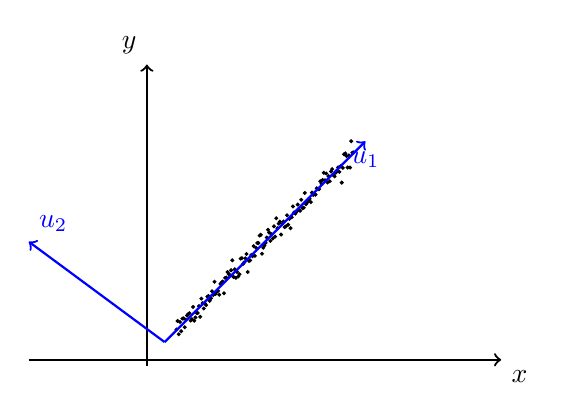
\begin{tikzpicture}[scale=0.75]
  \foreach \x/\y in {0.5/0.511870677093,0.520134228188/0.657474112041,0.540268456376/0.433301054831,0.560402684564/0.639402738784,0.580536912752/0.484888418032,0.60067114094/0.698401610126,0.620805369128/0.7012649978,0.640939597315/0.550258599782,0.661073825503/0.678863257247,0.681208053691/0.75063942818,0.701342281879/0.776722844493,0.721476510067/0.787974629261,0.741610738255/0.664867942136,0.761744966443/0.686496368534,0.781879194631/0.895235993285,0.802013422819/0.661601738133,0.822147651007/0.717376222072,0.842281879195/0.796219038444,0.862416107383/0.792290066926,0.88255033557/0.908555964509,0.902684563758/0.728213610997,0.922818791946/1.03682525621,0.942953020134/0.959254604949,0.963087248322/0.868395203865,0.98322147651/0.954903379431,1.0033557047/0.925500701421,1.02348993289/1.0700072327,1.04362416107/1.07910784654,1.06375838926/0.998680883498,1.08389261745/1.04215184899,1.10402684564/1.15961695354,1.12416107383/1.09641078989,1.14429530201/1.32135817413,1.1644295302/1.11554678055,1.18456375839/1.15881333579,1.20469798658/1.16650720076,1.22483221477/1.10170000196,1.24496644295/1.2856802819,1.26510067114/1.31032588214,1.28523489933/1.32664087434,1.30536912752/1.12586374789,1.3255033557/1.38744778116,1.34563758389/1.39149477354,1.36577181208/1.4858410387,1.38590604027/1.45489220706,1.40604026846/1.42066727608,1.42617449664/1.51638552543,1.44630872483/1.68453235672,1.46644295302/1.40404774902,1.48657718121/1.53217972768,1.5067114094/1.38840003053,1.52684563758/1.48738732887,1.54697986577/1.40903699426,1.56711409396/1.44846302024,1.58724832215/1.71184821717,1.60738255034/1.72156284303,1.62751677852/1.62088209802,1.64765100671/1.64829634188,1.6677852349/1.71789690662,1.68791946309/1.79158703578,1.70805369128/1.4865801932,1.72818791946/1.67235453921,1.74832214765/1.68309131722,1.76845637584/1.77403777092,1.78859060403/1.75540229337,1.80872483221/1.92421819935,1.8288590604/1.76070413373,1.84899328859/1.89440714397,1.86912751678/1.97867095812,1.88926174497/1.9767064361,1.90939597315/2.10350092601,1.92953020134/2.11726782381,1.94966442953/1.79668775603,1.96979865772/1.8979484069,1.98993288591/1.93277217634,2.01006711409/1.97986856224,2.03020134228/2.07115112966,2.05033557047/2.20256198706,2.07046979866/2.15486115796,2.09060402685/2.0135265175,2.11073825503/2.12456025274,2.13087248322/2.05492034879,2.15100671141/2.26017076362,2.1711409396/2.08564641805,2.19127516779/2.39746927122,2.21140939597/2.22522490056,2.23154362416/2.30668911212,2.25167785235/2.3405336089,2.27181208054/2.12057378128,2.29194630872/2.30428172148,2.31208053691/2.34209297556,2.3322147651/2.24731114226,2.35234899329/2.25863238242,2.37248322148/2.44749889836,2.39261744966/2.28794979535,2.41275167785/2.38637728425,2.43288590604/2.22855717892,2.45302013423/2.41476899048,2.47315436242/2.59725934406,2.4932885906/2.49509909292,2.51342281879/2.475381467,2.53355704698/2.50849761644,2.55369127517/2.62894898586,2.57382550336/2.53964404005,2.59395973154/2.52304084678,2.61409395973/2.71120042668,2.63422818792/2.56659063768,2.65436241611/2.57507058482,2.6744966443/2.82455379784,2.69463087248/2.63449675455,2.71476510067/2.66520230501,2.73489932886/2.70961994446,2.75503355705/2.72467839298,2.77516778523/2.67053791754,2.79530201342/2.83185765234,2.81543624161/2.79124434869,2.8355704698/2.81620859231,2.85570469799/2.79664069335,2.87583892617/2.90595671478,2.89597315436/2.88803599738,2.91610738255/2.89044757658,2.93624161074/3.02268962114,2.95637583893/2.98120872379,2.97651006711/3.04538380829,2.9966442953/3.16677251227,3.01677852349/3.03954291368,3.03691275168/3.15577291285,3.05704697987/3.00237643869,3.07718120805/3.10771652408,3.09731543624/3.02357015434,3.11744966443/3.18830966895,3.13758389262/3.22886917638,3.15771812081/3.12806798086,3.17785234899/3.10674403454,3.19798657718/3.16730762796,3.21812080537/3.19780291521,3.23825503356/3.25800939012,3.25838926174/3.18329683084,3.27852348993/3.27555040698,3.3/3,3.31879194631/3.24878603874,3.3389261745/3.48010644439,3.35906040268/3.49488774085,3.37919463087/3.45169839488,3.39932885906/3.2562776487,3.41946308725/3.45982610179,3.43959731544/3.25489013156,3.45973154362/3.70199350258,3.47986577181/3.50720556225,3.5/3.51067497333}
    {
      \node at (\x,\y)[circle,draw=black,fill=black,inner sep=0pt,minimum size=0.35mm]{};
    }
  \draw [thick, black, ->] (-2,0) -- (6, 0) node[anchor=north west] {$x$};
  \draw [thick, black, ->] (0,-0.1) -- (0, 5) node[anchor=south east] {$y$};
  \draw [thick,blue,->] (0.3,0.3) -- (3.7,3.7) node[anchor=north]{$u_1$};
  \draw [thick,blue,->] (0.3,0.3) -- (-2,2) node[anchor=south west]{$u_2$};
\end{tikzpicture}
}
\savestack{\pcacolor}{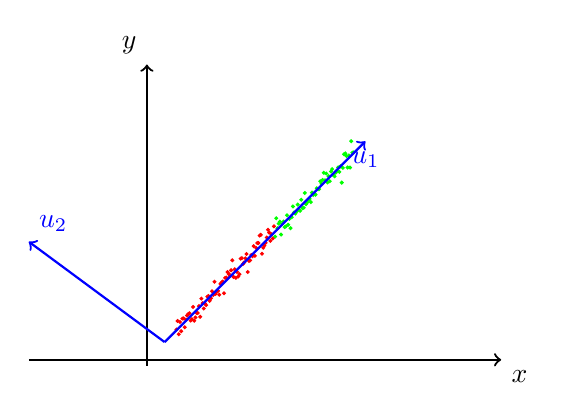
\begin{tikzpicture}[scale=0.75]
  \foreach \x/\y in {2.1711409396/2.08564641805,2.19127516779/2.39746927122,2.21140939597/2.22522490056,2.23154362416/2.30668911212,2.25167785235/2.3405336089,2.27181208054/2.12057378128,2.29194630872/2.30428172148,2.31208053691/2.34209297556,2.3322147651/2.24731114226,2.35234899329/2.25863238242,2.37248322148/2.44749889836,2.39261744966/2.28794979535,2.41275167785/2.38637728425,2.43288590604/2.22855717892,2.45302013423/2.41476899048,2.47315436242/2.59725934406,2.4932885906/2.49509909292,2.51342281879/2.475381467,2.53355704698/2.50849761644,2.55369127517/2.62894898586,2.57382550336/2.53964404005,2.59395973154/2.52304084678,2.61409395973/2.71120042668,2.63422818792/2.56659063768,2.65436241611/2.57507058482,2.6744966443/2.82455379784,2.69463087248/2.63449675455,2.71476510067/2.66520230501,2.73489932886/2.70961994446,2.75503355705/2.72467839298,2.77516778523/2.67053791754,2.79530201342/2.83185765234,2.81543624161/2.79124434869,2.8355704698/2.81620859231,2.85570469799/2.79664069335,2.87583892617/2.90595671478,2.89597315436/2.88803599738,2.91610738255/2.89044757658,2.93624161074/3.02268962114,2.95637583893/2.98120872379,2.97651006711/3.04538380829,2.9966442953/3.16677251227,3.01677852349/3.03954291368,3.03691275168/3.15577291285,3.05704697987/3.00237643869,3.07718120805/3.10771652408,3.09731543624/3.02357015434,3.11744966443/3.18830966895,3.13758389262/3.22886917638,3.15771812081/3.12806798086,3.17785234899/3.10674403454,3.19798657718/3.16730762796,3.21812080537/3.19780291521,3.23825503356/3.25800939012,3.25838926174/3.18329683084,3.27852348993/3.27555040698,3.3/3,3.31879194631/3.24878603874,3.3389261745/3.48010644439,3.35906040268/3.49488774085,3.37919463087/3.45169839488,3.39932885906/3.2562776487,3.41946308725/3.45982610179,3.43959731544/3.25489013156,3.45973154362/3.70199350258,3.47986577181/3.50720556225,3.5/3.51067497333}
    {
      \node at (\x,\y)[circle,draw=green,fill=green,inner sep=0pt,minimum size=0.35mm]{};
    }
  \foreach \x/\y in
    {0.5/0.511870677093,0.520134228188/0.657474112041,0.540268456376/0.433301054831,0.560402684564/0.639402738784,0.580536912752/0.484888418032,0.60067114094/0.698401610126,0.620805369128/0.7012649978,0.640939597315/0.550258599782,0.661073825503/0.678863257247,0.681208053691/0.75063942818,0.701342281879/0.776722844493,0.721476510067/0.787974629261,0.741610738255/0.664867942136,0.761744966443/0.686496368534,0.781879194631/0.895235993285,0.802013422819/0.661601738133,0.822147651007/0.717376222072,0.842281879195/0.796219038444,0.862416107383/0.792290066926,0.88255033557/0.908555964509,0.902684563758/0.728213610997,0.922818791946/1.03682525621,0.942953020134/0.959254604949,0.963087248322/0.868395203865,0.98322147651/0.954903379431,1.0033557047/0.925500701421,1.02348993289/1.0700072327,1.04362416107/1.07910784654,1.06375838926/0.998680883498,1.08389261745/1.04215184899,1.10402684564/1.15961695354,1.12416107383/1.09641078989,1.14429530201/1.32135817413,1.1644295302/1.11554678055,1.18456375839/1.15881333579,1.20469798658/1.16650720076,1.22483221477/1.10170000196,1.24496644295/1.2856802819,1.26510067114/1.31032588214,1.28523489933/1.32664087434,1.30536912752/1.12586374789,1.3255033557/1.38744778116,1.34563758389/1.39149477354,1.36577181208/1.4858410387,1.38590604027/1.45489220706,1.40604026846/1.42066727608,1.42617449664/1.51638552543,1.44630872483/1.68453235672,1.46644295302/1.40404774902,1.48657718121/1.53217972768,1.5067114094/1.38840003053,1.52684563758/1.48738732887,1.54697986577/1.40903699426,1.56711409396/1.44846302024,1.58724832215/1.71184821717,1.60738255034/1.72156284303,1.62751677852/1.62088209802,1.64765100671/1.64829634188,1.6677852349/1.71789690662,1.68791946309/1.79158703578,1.70805369128/1.4865801932,1.72818791946/1.67235453921,1.74832214765/1.68309131722,1.76845637584/1.77403777092,1.78859060403/1.75540229337,1.80872483221/1.92421819935,1.8288590604/1.76070413373,1.84899328859/1.89440714397,1.86912751678/1.97867095812,1.88926174497/1.9767064361,1.90939597315/2.10350092601,1.92953020134/2.11726782381,1.94966442953/1.79668775603,1.96979865772/1.8979484069,1.98993288591/1.93277217634,2.01006711409/1.97986856224,2.03020134228/2.07115112966,2.05033557047/2.20256198706,2.07046979866/2.15486115796,2.09060402685/2.0135265175,2.11073825503/2.12456025274,2.13087248322/2.05492034879,2.15100671141/2.26017076362
    }
    {
      \node at (\x,\y)[circle,draw=red,fill=red,inner sep=0pt,minimum size=0.35mm]{};
    }
  \draw [thick, black, ->] (-2,0) -- (6, 0) node[anchor=north west] {$x$};
  \draw [thick, black, ->] (0,-0.1) -- (0, 5) node[anchor=south east] {$y$};
  \draw [thick,blue,->] (0.3,0.3) -- (3.7,3.7) node[anchor=north]{$u_1$};
  \draw [thick,blue,->] (0.3,0.3) -- (-2,2) node[anchor=south west]{$u_2$};
\end{tikzpicture}
}

\begin{frame}
  \myheading{Module 6.4 : Principal Component Analysis and its Interpretations}
\end{frame}

% Slide 24
\begin{frame}
  \begin{block}{The story ahead...}
    \begin{itemize}\justifying
      \item<2-> \onslide<2->{Over the next few slides we will introduce Principal Component Analysis and see three different interpretations of it}
    \end{itemize}
  \end{block}
\end{frame}



%-----------------------------------------------------------------------------------------------------------
% Slide 25
\begin{frame}
  \begin{columns}
    \column{0.5\textwidth}
    \begin{overlayarea}{\textwidth}{\textheight}
      \makebox[\textwidth][c]{\usebox{\pcabnwnoaxiscontent}}
      % \begin{tikzpicture}[scale=0.75]
  \foreach \x/\y in {0.5/0.511870677093,0.520134228188/0.657474112041,0.540268456376/0.433301054831,0.560402684564/0.639402738784,0.580536912752/0.484888418032,0.60067114094/0.698401610126,0.620805369128/0.7012649978,0.640939597315/0.550258599782,0.661073825503/0.678863257247,0.681208053691/0.75063942818,0.701342281879/0.776722844493,0.721476510067/0.787974629261,0.741610738255/0.664867942136,0.761744966443/0.686496368534,0.781879194631/0.895235993285,0.802013422819/0.661601738133,0.822147651007/0.717376222072,0.842281879195/0.796219038444,0.862416107383/0.792290066926,0.88255033557/0.908555964509,0.902684563758/0.728213610997,0.922818791946/1.03682525621,0.942953020134/0.959254604949,0.963087248322/0.868395203865,0.98322147651/0.954903379431,1.0033557047/0.925500701421,1.02348993289/1.0700072327,1.04362416107/1.07910784654,1.06375838926/0.998680883498,1.08389261745/1.04215184899,1.10402684564/1.15961695354,1.12416107383/1.09641078989,1.14429530201/1.32135817413,1.1644295302/1.11554678055,1.18456375839/1.15881333579,1.20469798658/1.16650720076,1.22483221477/1.10170000196,1.24496644295/1.2856802819,1.26510067114/1.31032588214,1.28523489933/1.32664087434,1.30536912752/1.12586374789,1.3255033557/1.38744778116,1.34563758389/1.39149477354,1.36577181208/1.4858410387,1.38590604027/1.45489220706,1.40604026846/1.42066727608,1.42617449664/1.51638552543,1.44630872483/1.68453235672,1.46644295302/1.40404774902,1.48657718121/1.53217972768,1.5067114094/1.38840003053,1.52684563758/1.48738732887,1.54697986577/1.40903699426,1.56711409396/1.44846302024,1.58724832215/1.71184821717,1.60738255034/1.72156284303,1.62751677852/1.62088209802,1.64765100671/1.64829634188,1.6677852349/1.71789690662,1.68791946309/1.79158703578,1.70805369128/1.4865801932,1.72818791946/1.67235453921,1.74832214765/1.68309131722,1.76845637584/1.77403777092,1.78859060403/1.75540229337,1.80872483221/1.92421819935,1.8288590604/1.76070413373,1.84899328859/1.89440714397,1.86912751678/1.97867095812,1.88926174497/1.9767064361,1.90939597315/2.10350092601,1.92953020134/2.11726782381,1.94966442953/1.79668775603,1.96979865772/1.8979484069,1.98993288591/1.93277217634,2.01006711409/1.97986856224,2.03020134228/2.07115112966,2.05033557047/2.20256198706,2.07046979866/2.15486115796,2.09060402685/2.0135265175,2.11073825503/2.12456025274,2.13087248322/2.05492034879,2.15100671141/2.26017076362,2.1711409396/2.08564641805,2.19127516779/2.39746927122,2.21140939597/2.22522490056,2.23154362416/2.30668911212,2.25167785235/2.3405336089,2.27181208054/2.12057378128,2.29194630872/2.30428172148,2.31208053691/2.34209297556,2.3322147651/2.24731114226,2.35234899329/2.25863238242,2.37248322148/2.44749889836,2.39261744966/2.28794979535,2.41275167785/2.38637728425,2.43288590604/2.22855717892,2.45302013423/2.41476899048,2.47315436242/2.59725934406,2.4932885906/2.49509909292,2.51342281879/2.475381467,2.53355704698/2.50849761644,2.55369127517/2.62894898586,2.57382550336/2.53964404005,2.59395973154/2.52304084678,2.61409395973/2.71120042668,2.63422818792/2.56659063768,2.65436241611/2.57507058482,2.6744966443/2.82455379784,2.69463087248/2.63449675455,2.71476510067/2.66520230501,2.73489932886/2.70961994446,2.75503355705/2.72467839298,2.77516778523/2.67053791754,2.79530201342/2.83185765234,2.81543624161/2.79124434869,2.8355704698/2.81620859231,2.85570469799/2.79664069335,2.87583892617/2.90595671478,2.89597315436/2.88803599738,2.91610738255/2.89044757658,2.93624161074/3.02268962114,2.95637583893/2.98120872379,2.97651006711/3.04538380829,2.9966442953/3.16677251227,3.01677852349/3.03954291368,3.03691275168/3.15577291285,3.05704697987/3.00237643869,3.07718120805/3.10771652408,3.09731543624/3.02357015434,3.11744966443/3.18830966895,3.13758389262/3.22886917638,3.15771812081/3.12806798086,3.17785234899/3.10674403454,3.19798657718/3.16730762796,3.21812080537/3.19780291521,3.23825503356/3.25800939012,3.25838926174/3.18329683084,3.27852348993/3.27555040698,3.3/3,3.31879194631/3.24878603874,3.3389261745/3.48010644439,3.35906040268/3.49488774085,3.37919463087/3.45169839488,3.39932885906/3.2562776487,3.41946308725/3.45982610179,3.43959731544/3.25489013156,3.45973154362/3.70199350258,3.47986577181/3.50720556225,3.5/3.51067497333}
    {
      \node at (\x,\y)[circle,draw=black,fill=black,inner sep=0pt,minimum size=0.35mm]{};
    }
  \draw [thick, black, ->] (-2,0) -- (6, 0) node[anchor=north west] {$x$};
  \draw [thick, black, ->] (0,-0.1) -- (0, 5) node[anchor=south east] {$y$};
\end{tikzpicture}

    \end{overlayarea}

    \column{0.5\textwidth}
    \begin{overlayarea}{\textwidth}{\textheight}
      \begin{itemize}\justifying
        \item<1-> Consider the following data
        \item<2-> Each point (vector) here is represented using a linear combination of the $x$ and $y$ axes (i.e. using the point's $x$ and $y$ co-ordinates)
        \item<3-> In other words we are using $x$ and $y$ as the basis
        \item<4-> What if we choose a different basis?
      \end{itemize}
    \end{overlayarea}
  \end{columns}
\end{frame}

%----------------------------------------------------------------------------------------------------------
% Slide 26
\begin{frame}
  \begin{columns}
    \column{0.5\textwidth}<1->
    \begin{overlayarea}{\textwidth}{\textheight}
      \makebox[\textwidth][c]{\usebox{\pcabnwaxiscontent}}
      % 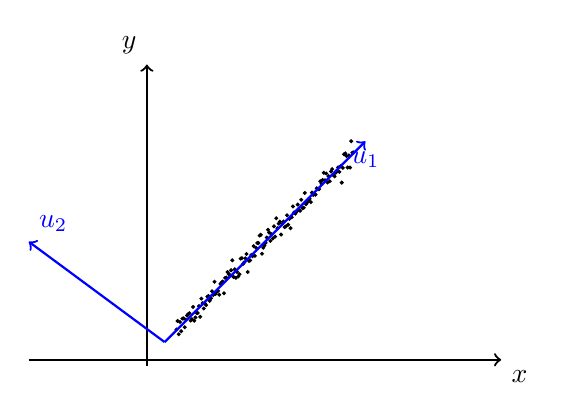
\begin{tikzpicture}[scale=0.75]
  \foreach \x/\y in {0.5/0.511870677093,0.520134228188/0.657474112041,0.540268456376/0.433301054831,0.560402684564/0.639402738784,0.580536912752/0.484888418032,0.60067114094/0.698401610126,0.620805369128/0.7012649978,0.640939597315/0.550258599782,0.661073825503/0.678863257247,0.681208053691/0.75063942818,0.701342281879/0.776722844493,0.721476510067/0.787974629261,0.741610738255/0.664867942136,0.761744966443/0.686496368534,0.781879194631/0.895235993285,0.802013422819/0.661601738133,0.822147651007/0.717376222072,0.842281879195/0.796219038444,0.862416107383/0.792290066926,0.88255033557/0.908555964509,0.902684563758/0.728213610997,0.922818791946/1.03682525621,0.942953020134/0.959254604949,0.963087248322/0.868395203865,0.98322147651/0.954903379431,1.0033557047/0.925500701421,1.02348993289/1.0700072327,1.04362416107/1.07910784654,1.06375838926/0.998680883498,1.08389261745/1.04215184899,1.10402684564/1.15961695354,1.12416107383/1.09641078989,1.14429530201/1.32135817413,1.1644295302/1.11554678055,1.18456375839/1.15881333579,1.20469798658/1.16650720076,1.22483221477/1.10170000196,1.24496644295/1.2856802819,1.26510067114/1.31032588214,1.28523489933/1.32664087434,1.30536912752/1.12586374789,1.3255033557/1.38744778116,1.34563758389/1.39149477354,1.36577181208/1.4858410387,1.38590604027/1.45489220706,1.40604026846/1.42066727608,1.42617449664/1.51638552543,1.44630872483/1.68453235672,1.46644295302/1.40404774902,1.48657718121/1.53217972768,1.5067114094/1.38840003053,1.52684563758/1.48738732887,1.54697986577/1.40903699426,1.56711409396/1.44846302024,1.58724832215/1.71184821717,1.60738255034/1.72156284303,1.62751677852/1.62088209802,1.64765100671/1.64829634188,1.6677852349/1.71789690662,1.68791946309/1.79158703578,1.70805369128/1.4865801932,1.72818791946/1.67235453921,1.74832214765/1.68309131722,1.76845637584/1.77403777092,1.78859060403/1.75540229337,1.80872483221/1.92421819935,1.8288590604/1.76070413373,1.84899328859/1.89440714397,1.86912751678/1.97867095812,1.88926174497/1.9767064361,1.90939597315/2.10350092601,1.92953020134/2.11726782381,1.94966442953/1.79668775603,1.96979865772/1.8979484069,1.98993288591/1.93277217634,2.01006711409/1.97986856224,2.03020134228/2.07115112966,2.05033557047/2.20256198706,2.07046979866/2.15486115796,2.09060402685/2.0135265175,2.11073825503/2.12456025274,2.13087248322/2.05492034879,2.15100671141/2.26017076362,2.1711409396/2.08564641805,2.19127516779/2.39746927122,2.21140939597/2.22522490056,2.23154362416/2.30668911212,2.25167785235/2.3405336089,2.27181208054/2.12057378128,2.29194630872/2.30428172148,2.31208053691/2.34209297556,2.3322147651/2.24731114226,2.35234899329/2.25863238242,2.37248322148/2.44749889836,2.39261744966/2.28794979535,2.41275167785/2.38637728425,2.43288590604/2.22855717892,2.45302013423/2.41476899048,2.47315436242/2.59725934406,2.4932885906/2.49509909292,2.51342281879/2.475381467,2.53355704698/2.50849761644,2.55369127517/2.62894898586,2.57382550336/2.53964404005,2.59395973154/2.52304084678,2.61409395973/2.71120042668,2.63422818792/2.56659063768,2.65436241611/2.57507058482,2.6744966443/2.82455379784,2.69463087248/2.63449675455,2.71476510067/2.66520230501,2.73489932886/2.70961994446,2.75503355705/2.72467839298,2.77516778523/2.67053791754,2.79530201342/2.83185765234,2.81543624161/2.79124434869,2.8355704698/2.81620859231,2.85570469799/2.79664069335,2.87583892617/2.90595671478,2.89597315436/2.88803599738,2.91610738255/2.89044757658,2.93624161074/3.02268962114,2.95637583893/2.98120872379,2.97651006711/3.04538380829,2.9966442953/3.16677251227,3.01677852349/3.03954291368,3.03691275168/3.15577291285,3.05704697987/3.00237643869,3.07718120805/3.10771652408,3.09731543624/3.02357015434,3.11744966443/3.18830966895,3.13758389262/3.22886917638,3.15771812081/3.12806798086,3.17785234899/3.10674403454,3.19798657718/3.16730762796,3.21812080537/3.19780291521,3.23825503356/3.25800939012,3.25838926174/3.18329683084,3.27852348993/3.27555040698,3.3/3,3.31879194631/3.24878603874,3.3389261745/3.48010644439,3.35906040268/3.49488774085,3.37919463087/3.45169839488,3.39932885906/3.2562776487,3.41946308725/3.45982610179,3.43959731544/3.25489013156,3.45973154362/3.70199350258,3.47986577181/3.50720556225,3.5/3.51067497333}
    {
      \node at (\x,\y)[circle,draw=black,fill=black,inner sep=0pt,minimum size=0.35mm]{};
    }
  \draw [thick, black, ->] (-2,0) -- (6, 0) node[anchor=north west] {$x$};
  \draw [thick, black, ->] (0,-0.1) -- (0, 5) node[anchor=south east] {$y$};
  \draw [thick,blue,->] (0.3,0.3) -- (3.7,3.7) node[anchor=north]{$u_1$};
  \draw [thick,blue,->] (0.3,0.3) -- (-2,2) node[anchor=south west]{$u_2$};
\end{tikzpicture}

    \end{overlayarea}

    \column{0.5\textwidth}<1->
    \begin{overlayarea}{\textwidth}{\textheight}
      \begin{itemize}\justifying
        \item<1-> For example, what if we use $u_1$ and $u_2$ as a basis instead of $x$ and $y$.
        \item<2-> We observe that all the points have a very small component in the direction of $u_2$ (almost noise)
        \item<3-> It seems that the same data which was originally in $\mathbb{R}^2(x,y)$ can now be represented in $\mathbb{R}^{1}(u_1)$ by making a smarter choice for the basis
      \end{itemize}
    \end{overlayarea}
  \end{columns}
\end{frame}

%----------------------------------------------------------------------------------------------------------
% Slide 27
\begin{frame}
  \begin{columns}
    \column{0.5\textwidth}<1->
    \begin{overlayarea}{\textwidth}{\textheight}
      \only<1-3>{\makebox[\textwidth][c]{\usebox{\pcabnwaxiscontent}}}
      \only<4->{\makebox[\textwidth][c]{\usebox{\pcacolorcontent}}}

      % \only<1-3>{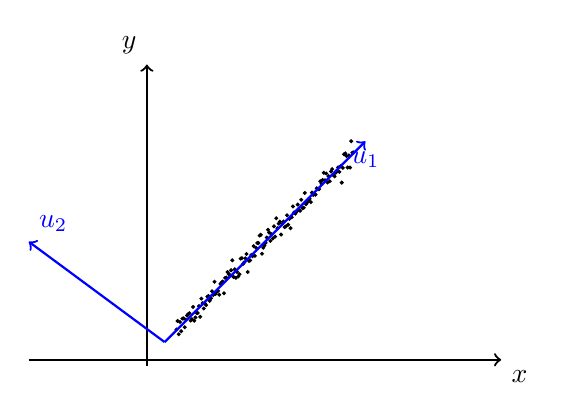
\begin{tikzpicture}[scale=0.75]
  \foreach \x/\y in {0.5/0.511870677093,0.520134228188/0.657474112041,0.540268456376/0.433301054831,0.560402684564/0.639402738784,0.580536912752/0.484888418032,0.60067114094/0.698401610126,0.620805369128/0.7012649978,0.640939597315/0.550258599782,0.661073825503/0.678863257247,0.681208053691/0.75063942818,0.701342281879/0.776722844493,0.721476510067/0.787974629261,0.741610738255/0.664867942136,0.761744966443/0.686496368534,0.781879194631/0.895235993285,0.802013422819/0.661601738133,0.822147651007/0.717376222072,0.842281879195/0.796219038444,0.862416107383/0.792290066926,0.88255033557/0.908555964509,0.902684563758/0.728213610997,0.922818791946/1.03682525621,0.942953020134/0.959254604949,0.963087248322/0.868395203865,0.98322147651/0.954903379431,1.0033557047/0.925500701421,1.02348993289/1.0700072327,1.04362416107/1.07910784654,1.06375838926/0.998680883498,1.08389261745/1.04215184899,1.10402684564/1.15961695354,1.12416107383/1.09641078989,1.14429530201/1.32135817413,1.1644295302/1.11554678055,1.18456375839/1.15881333579,1.20469798658/1.16650720076,1.22483221477/1.10170000196,1.24496644295/1.2856802819,1.26510067114/1.31032588214,1.28523489933/1.32664087434,1.30536912752/1.12586374789,1.3255033557/1.38744778116,1.34563758389/1.39149477354,1.36577181208/1.4858410387,1.38590604027/1.45489220706,1.40604026846/1.42066727608,1.42617449664/1.51638552543,1.44630872483/1.68453235672,1.46644295302/1.40404774902,1.48657718121/1.53217972768,1.5067114094/1.38840003053,1.52684563758/1.48738732887,1.54697986577/1.40903699426,1.56711409396/1.44846302024,1.58724832215/1.71184821717,1.60738255034/1.72156284303,1.62751677852/1.62088209802,1.64765100671/1.64829634188,1.6677852349/1.71789690662,1.68791946309/1.79158703578,1.70805369128/1.4865801932,1.72818791946/1.67235453921,1.74832214765/1.68309131722,1.76845637584/1.77403777092,1.78859060403/1.75540229337,1.80872483221/1.92421819935,1.8288590604/1.76070413373,1.84899328859/1.89440714397,1.86912751678/1.97867095812,1.88926174497/1.9767064361,1.90939597315/2.10350092601,1.92953020134/2.11726782381,1.94966442953/1.79668775603,1.96979865772/1.8979484069,1.98993288591/1.93277217634,2.01006711409/1.97986856224,2.03020134228/2.07115112966,2.05033557047/2.20256198706,2.07046979866/2.15486115796,2.09060402685/2.0135265175,2.11073825503/2.12456025274,2.13087248322/2.05492034879,2.15100671141/2.26017076362,2.1711409396/2.08564641805,2.19127516779/2.39746927122,2.21140939597/2.22522490056,2.23154362416/2.30668911212,2.25167785235/2.3405336089,2.27181208054/2.12057378128,2.29194630872/2.30428172148,2.31208053691/2.34209297556,2.3322147651/2.24731114226,2.35234899329/2.25863238242,2.37248322148/2.44749889836,2.39261744966/2.28794979535,2.41275167785/2.38637728425,2.43288590604/2.22855717892,2.45302013423/2.41476899048,2.47315436242/2.59725934406,2.4932885906/2.49509909292,2.51342281879/2.475381467,2.53355704698/2.50849761644,2.55369127517/2.62894898586,2.57382550336/2.53964404005,2.59395973154/2.52304084678,2.61409395973/2.71120042668,2.63422818792/2.56659063768,2.65436241611/2.57507058482,2.6744966443/2.82455379784,2.69463087248/2.63449675455,2.71476510067/2.66520230501,2.73489932886/2.70961994446,2.75503355705/2.72467839298,2.77516778523/2.67053791754,2.79530201342/2.83185765234,2.81543624161/2.79124434869,2.8355704698/2.81620859231,2.85570469799/2.79664069335,2.87583892617/2.90595671478,2.89597315436/2.88803599738,2.91610738255/2.89044757658,2.93624161074/3.02268962114,2.95637583893/2.98120872379,2.97651006711/3.04538380829,2.9966442953/3.16677251227,3.01677852349/3.03954291368,3.03691275168/3.15577291285,3.05704697987/3.00237643869,3.07718120805/3.10771652408,3.09731543624/3.02357015434,3.11744966443/3.18830966895,3.13758389262/3.22886917638,3.15771812081/3.12806798086,3.17785234899/3.10674403454,3.19798657718/3.16730762796,3.21812080537/3.19780291521,3.23825503356/3.25800939012,3.25838926174/3.18329683084,3.27852348993/3.27555040698,3.3/3,3.31879194631/3.24878603874,3.3389261745/3.48010644439,3.35906040268/3.49488774085,3.37919463087/3.45169839488,3.39932885906/3.2562776487,3.41946308725/3.45982610179,3.43959731544/3.25489013156,3.45973154362/3.70199350258,3.47986577181/3.50720556225,3.5/3.51067497333}
    {
      \node at (\x,\y)[circle,draw=black,fill=black,inner sep=0pt,minimum size=0.35mm]{};
    }
  \draw [thick, black, ->] (-2,0) -- (6, 0) node[anchor=north west] {$x$};
  \draw [thick, black, ->] (0,-0.1) -- (0, 5) node[anchor=south east] {$y$};
  \draw [thick,blue,->] (0.3,0.3) -- (3.7,3.7) node[anchor=north]{$u_1$};
  \draw [thick,blue,->] (0.3,0.3) -- (-2,2) node[anchor=south west]{$u_2$};
\end{tikzpicture}
}
      % \only<4->{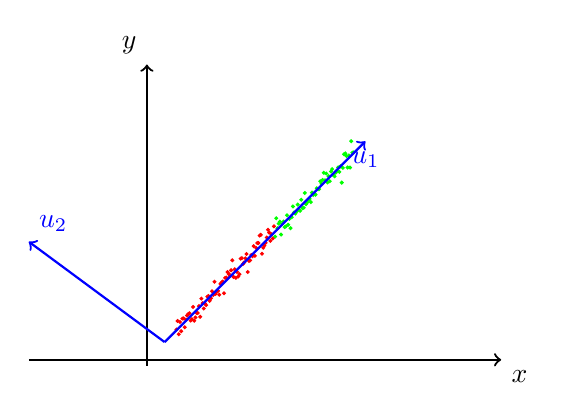
\begin{tikzpicture}[scale=0.75]
  \foreach \x/\y in {2.1711409396/2.08564641805,2.19127516779/2.39746927122,2.21140939597/2.22522490056,2.23154362416/2.30668911212,2.25167785235/2.3405336089,2.27181208054/2.12057378128,2.29194630872/2.30428172148,2.31208053691/2.34209297556,2.3322147651/2.24731114226,2.35234899329/2.25863238242,2.37248322148/2.44749889836,2.39261744966/2.28794979535,2.41275167785/2.38637728425,2.43288590604/2.22855717892,2.45302013423/2.41476899048,2.47315436242/2.59725934406,2.4932885906/2.49509909292,2.51342281879/2.475381467,2.53355704698/2.50849761644,2.55369127517/2.62894898586,2.57382550336/2.53964404005,2.59395973154/2.52304084678,2.61409395973/2.71120042668,2.63422818792/2.56659063768,2.65436241611/2.57507058482,2.6744966443/2.82455379784,2.69463087248/2.63449675455,2.71476510067/2.66520230501,2.73489932886/2.70961994446,2.75503355705/2.72467839298,2.77516778523/2.67053791754,2.79530201342/2.83185765234,2.81543624161/2.79124434869,2.8355704698/2.81620859231,2.85570469799/2.79664069335,2.87583892617/2.90595671478,2.89597315436/2.88803599738,2.91610738255/2.89044757658,2.93624161074/3.02268962114,2.95637583893/2.98120872379,2.97651006711/3.04538380829,2.9966442953/3.16677251227,3.01677852349/3.03954291368,3.03691275168/3.15577291285,3.05704697987/3.00237643869,3.07718120805/3.10771652408,3.09731543624/3.02357015434,3.11744966443/3.18830966895,3.13758389262/3.22886917638,3.15771812081/3.12806798086,3.17785234899/3.10674403454,3.19798657718/3.16730762796,3.21812080537/3.19780291521,3.23825503356/3.25800939012,3.25838926174/3.18329683084,3.27852348993/3.27555040698,3.3/3,3.31879194631/3.24878603874,3.3389261745/3.48010644439,3.35906040268/3.49488774085,3.37919463087/3.45169839488,3.39932885906/3.2562776487,3.41946308725/3.45982610179,3.43959731544/3.25489013156,3.45973154362/3.70199350258,3.47986577181/3.50720556225,3.5/3.51067497333}
    {
      \node at (\x,\y)[circle,draw=green,fill=green,inner sep=0pt,minimum size=0.35mm]{};
    }
  \foreach \x/\y in
    {0.5/0.511870677093,0.520134228188/0.657474112041,0.540268456376/0.433301054831,0.560402684564/0.639402738784,0.580536912752/0.484888418032,0.60067114094/0.698401610126,0.620805369128/0.7012649978,0.640939597315/0.550258599782,0.661073825503/0.678863257247,0.681208053691/0.75063942818,0.701342281879/0.776722844493,0.721476510067/0.787974629261,0.741610738255/0.664867942136,0.761744966443/0.686496368534,0.781879194631/0.895235993285,0.802013422819/0.661601738133,0.822147651007/0.717376222072,0.842281879195/0.796219038444,0.862416107383/0.792290066926,0.88255033557/0.908555964509,0.902684563758/0.728213610997,0.922818791946/1.03682525621,0.942953020134/0.959254604949,0.963087248322/0.868395203865,0.98322147651/0.954903379431,1.0033557047/0.925500701421,1.02348993289/1.0700072327,1.04362416107/1.07910784654,1.06375838926/0.998680883498,1.08389261745/1.04215184899,1.10402684564/1.15961695354,1.12416107383/1.09641078989,1.14429530201/1.32135817413,1.1644295302/1.11554678055,1.18456375839/1.15881333579,1.20469798658/1.16650720076,1.22483221477/1.10170000196,1.24496644295/1.2856802819,1.26510067114/1.31032588214,1.28523489933/1.32664087434,1.30536912752/1.12586374789,1.3255033557/1.38744778116,1.34563758389/1.39149477354,1.36577181208/1.4858410387,1.38590604027/1.45489220706,1.40604026846/1.42066727608,1.42617449664/1.51638552543,1.44630872483/1.68453235672,1.46644295302/1.40404774902,1.48657718121/1.53217972768,1.5067114094/1.38840003053,1.52684563758/1.48738732887,1.54697986577/1.40903699426,1.56711409396/1.44846302024,1.58724832215/1.71184821717,1.60738255034/1.72156284303,1.62751677852/1.62088209802,1.64765100671/1.64829634188,1.6677852349/1.71789690662,1.68791946309/1.79158703578,1.70805369128/1.4865801932,1.72818791946/1.67235453921,1.74832214765/1.68309131722,1.76845637584/1.77403777092,1.78859060403/1.75540229337,1.80872483221/1.92421819935,1.8288590604/1.76070413373,1.84899328859/1.89440714397,1.86912751678/1.97867095812,1.88926174497/1.9767064361,1.90939597315/2.10350092601,1.92953020134/2.11726782381,1.94966442953/1.79668775603,1.96979865772/1.8979484069,1.98993288591/1.93277217634,2.01006711409/1.97986856224,2.03020134228/2.07115112966,2.05033557047/2.20256198706,2.07046979866/2.15486115796,2.09060402685/2.0135265175,2.11073825503/2.12456025274,2.13087248322/2.05492034879,2.15100671141/2.26017076362
    }
    {
      \node at (\x,\y)[circle,draw=red,fill=red,inner sep=0pt,minimum size=0.35mm]{};
    }
  \draw [thick, black, ->] (-2,0) -- (6, 0) node[anchor=north west] {$x$};
  \draw [thick, black, ->] (0,-0.1) -- (0, 5) node[anchor=south east] {$y$};
  \draw [thick,blue,->] (0.3,0.3) -- (3.7,3.7) node[anchor=north]{$u_1$};
  \draw [thick,blue,->] (0.3,0.3) -- (-2,2) node[anchor=south west]{$u_2$};
\end{tikzpicture}
}
    \end{overlayarea}

    \column{0.5\textwidth}<1->
    \begin{overlayarea}{\textwidth}{\textheight}
      \begin{itemize}\justifying
        \item<1-> Let's try stating this more formally
        \item<2-> Why do we not care about $u_2$?
        \item<3-> Because the variance in the data in this direction is very small (all data points have almost the same value in the $u_2$ direction)
        \item<4-> If we were to build a classifier on top of this data then $u_2$ would not contribute to the classifier as the points are not distinguishable along this direction
      \end{itemize}
    \end{overlayarea}
  \end{columns}
\end{frame}

%----------------------------------------------------------------------------------------------------------
% Slide 28
\begin{frame}
  \begin{columns}
    \column{0.5\textwidth}<1->
    \begin{overlayarea}{\textwidth}{\textheight}
      \makebox[\textwidth][c]{\usebox{\pcacolorcontent}}
     % 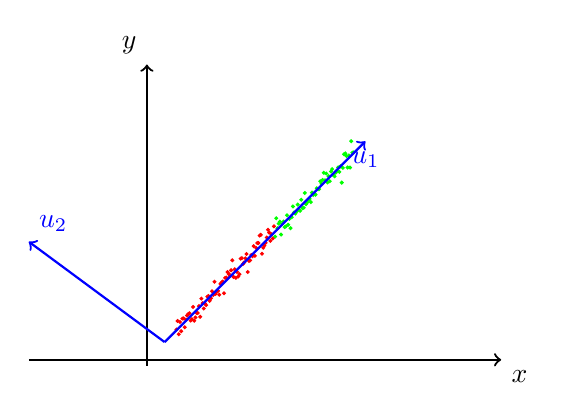
\begin{tikzpicture}[scale=0.75]
  \foreach \x/\y in {2.1711409396/2.08564641805,2.19127516779/2.39746927122,2.21140939597/2.22522490056,2.23154362416/2.30668911212,2.25167785235/2.3405336089,2.27181208054/2.12057378128,2.29194630872/2.30428172148,2.31208053691/2.34209297556,2.3322147651/2.24731114226,2.35234899329/2.25863238242,2.37248322148/2.44749889836,2.39261744966/2.28794979535,2.41275167785/2.38637728425,2.43288590604/2.22855717892,2.45302013423/2.41476899048,2.47315436242/2.59725934406,2.4932885906/2.49509909292,2.51342281879/2.475381467,2.53355704698/2.50849761644,2.55369127517/2.62894898586,2.57382550336/2.53964404005,2.59395973154/2.52304084678,2.61409395973/2.71120042668,2.63422818792/2.56659063768,2.65436241611/2.57507058482,2.6744966443/2.82455379784,2.69463087248/2.63449675455,2.71476510067/2.66520230501,2.73489932886/2.70961994446,2.75503355705/2.72467839298,2.77516778523/2.67053791754,2.79530201342/2.83185765234,2.81543624161/2.79124434869,2.8355704698/2.81620859231,2.85570469799/2.79664069335,2.87583892617/2.90595671478,2.89597315436/2.88803599738,2.91610738255/2.89044757658,2.93624161074/3.02268962114,2.95637583893/2.98120872379,2.97651006711/3.04538380829,2.9966442953/3.16677251227,3.01677852349/3.03954291368,3.03691275168/3.15577291285,3.05704697987/3.00237643869,3.07718120805/3.10771652408,3.09731543624/3.02357015434,3.11744966443/3.18830966895,3.13758389262/3.22886917638,3.15771812081/3.12806798086,3.17785234899/3.10674403454,3.19798657718/3.16730762796,3.21812080537/3.19780291521,3.23825503356/3.25800939012,3.25838926174/3.18329683084,3.27852348993/3.27555040698,3.3/3,3.31879194631/3.24878603874,3.3389261745/3.48010644439,3.35906040268/3.49488774085,3.37919463087/3.45169839488,3.39932885906/3.2562776487,3.41946308725/3.45982610179,3.43959731544/3.25489013156,3.45973154362/3.70199350258,3.47986577181/3.50720556225,3.5/3.51067497333}
    {
      \node at (\x,\y)[circle,draw=green,fill=green,inner sep=0pt,minimum size=0.35mm]{};
    }
  \foreach \x/\y in
    {0.5/0.511870677093,0.520134228188/0.657474112041,0.540268456376/0.433301054831,0.560402684564/0.639402738784,0.580536912752/0.484888418032,0.60067114094/0.698401610126,0.620805369128/0.7012649978,0.640939597315/0.550258599782,0.661073825503/0.678863257247,0.681208053691/0.75063942818,0.701342281879/0.776722844493,0.721476510067/0.787974629261,0.741610738255/0.664867942136,0.761744966443/0.686496368534,0.781879194631/0.895235993285,0.802013422819/0.661601738133,0.822147651007/0.717376222072,0.842281879195/0.796219038444,0.862416107383/0.792290066926,0.88255033557/0.908555964509,0.902684563758/0.728213610997,0.922818791946/1.03682525621,0.942953020134/0.959254604949,0.963087248322/0.868395203865,0.98322147651/0.954903379431,1.0033557047/0.925500701421,1.02348993289/1.0700072327,1.04362416107/1.07910784654,1.06375838926/0.998680883498,1.08389261745/1.04215184899,1.10402684564/1.15961695354,1.12416107383/1.09641078989,1.14429530201/1.32135817413,1.1644295302/1.11554678055,1.18456375839/1.15881333579,1.20469798658/1.16650720076,1.22483221477/1.10170000196,1.24496644295/1.2856802819,1.26510067114/1.31032588214,1.28523489933/1.32664087434,1.30536912752/1.12586374789,1.3255033557/1.38744778116,1.34563758389/1.39149477354,1.36577181208/1.4858410387,1.38590604027/1.45489220706,1.40604026846/1.42066727608,1.42617449664/1.51638552543,1.44630872483/1.68453235672,1.46644295302/1.40404774902,1.48657718121/1.53217972768,1.5067114094/1.38840003053,1.52684563758/1.48738732887,1.54697986577/1.40903699426,1.56711409396/1.44846302024,1.58724832215/1.71184821717,1.60738255034/1.72156284303,1.62751677852/1.62088209802,1.64765100671/1.64829634188,1.6677852349/1.71789690662,1.68791946309/1.79158703578,1.70805369128/1.4865801932,1.72818791946/1.67235453921,1.74832214765/1.68309131722,1.76845637584/1.77403777092,1.78859060403/1.75540229337,1.80872483221/1.92421819935,1.8288590604/1.76070413373,1.84899328859/1.89440714397,1.86912751678/1.97867095812,1.88926174497/1.9767064361,1.90939597315/2.10350092601,1.92953020134/2.11726782381,1.94966442953/1.79668775603,1.96979865772/1.8979484069,1.98993288591/1.93277217634,2.01006711409/1.97986856224,2.03020134228/2.07115112966,2.05033557047/2.20256198706,2.07046979866/2.15486115796,2.09060402685/2.0135265175,2.11073825503/2.12456025274,2.13087248322/2.05492034879,2.15100671141/2.26017076362
    }
    {
      \node at (\x,\y)[circle,draw=red,fill=red,inner sep=0pt,minimum size=0.35mm]{};
    }
  \draw [thick, black, ->] (-2,0) -- (6, 0) node[anchor=north west] {$x$};
  \draw [thick, black, ->] (0,-0.1) -- (0, 5) node[anchor=south east] {$y$};
  \draw [thick,blue,->] (0.3,0.3) -- (3.7,3.7) node[anchor=north]{$u_1$};
  \draw [thick,blue,->] (0.3,0.3) -- (-2,2) node[anchor=south west]{$u_2$};
\end{tikzpicture}

    \end{overlayarea}

    \column{0.5\textwidth}<1->
    \begin{overlayarea}{\textwidth}{\textheight}
      \begin{itemize}\justifying
        \item<1-> In general, we are interested in representing the data using fewer dimensions such that \onslide<2-> {the data has high variance along these dimensions}
        \item<3-> Is that all?
        \item<4-> No, there is something else that we desire. Let's see what.
      \end{itemize}
    \end{overlayarea}
  \end{columns}
\end{frame}

%----------------------------------------------------------------------------------------------------------
% Slide 29
\begin{frame}
  \begin{columns}
    \column{0.5\textwidth}<1->
    \begin{overlayarea}{\textwidth}{\textheight}
      \begin{table}[]
        \centering

        \label{my-label}
        \begin{tabular}{ccc}
          \hline
          \textbf{x} & \textbf{y} & \textbf{z} \\ \hline
          1          & 1          & 1          \\
          0.5        & 0          & 0          \\
          0.25       & 1          & 1          \\
          0.35       & 1.5        & 1.5        \\
          0.45       & 1          & 1          \\
          0.57       & 2          & 2.1        \\
          0.62       & 1.1        & 1          \\
          0.73       & 0.75       & 0.76       \\
          0.72       & 0.86       & 0.87       \\
          \hline
        \end{tabular}
      \end{table}
      \onslide<3->{
        \begin{equation*}
          \rho_{yz} = \frac{\sum_{i=1}^{n}(y_i-\overline{y})(z_i-\overline{z})}{\sqrt{\sum_{i=1}^{n}(y_i-\overline{y})^2}\sqrt{\sum_{i=1}^{n}(z_i-\overline{z})^2}}
        \end{equation*}
      }
    \end{overlayarea}

    \column{0.5\textwidth}<1->
    \begin{overlayarea}{\textwidth}{\textheight}
      \begin{itemize}\justifying
        \item<1-> Consider the following data
        \item<2-> Is $z$ adding any new information beyond what is already contained in $y$?
        \item<3-> The two columns are highly correlated (or they have a high covariance)
        \item<4-> In other words the column $z$ is redundant since it is linearly dependent on $y$.
      \end{itemize}
    \end{overlayarea}
  \end{columns}
\end{frame}

%----------------------------------------------------------------------------------------------------------
% Slide 30
\begin{frame}
  \begin{columns}
    \column{0.5\textwidth}<1->
    \begin{overlayarea}{\textwidth}{\textheight}
      \makebox[\textwidth][c]{\usebox{\pcacolorcontent}}
     % 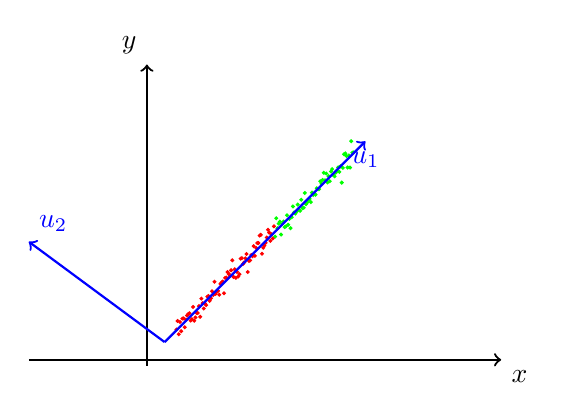
\begin{tikzpicture}[scale=0.75]
  \foreach \x/\y in {2.1711409396/2.08564641805,2.19127516779/2.39746927122,2.21140939597/2.22522490056,2.23154362416/2.30668911212,2.25167785235/2.3405336089,2.27181208054/2.12057378128,2.29194630872/2.30428172148,2.31208053691/2.34209297556,2.3322147651/2.24731114226,2.35234899329/2.25863238242,2.37248322148/2.44749889836,2.39261744966/2.28794979535,2.41275167785/2.38637728425,2.43288590604/2.22855717892,2.45302013423/2.41476899048,2.47315436242/2.59725934406,2.4932885906/2.49509909292,2.51342281879/2.475381467,2.53355704698/2.50849761644,2.55369127517/2.62894898586,2.57382550336/2.53964404005,2.59395973154/2.52304084678,2.61409395973/2.71120042668,2.63422818792/2.56659063768,2.65436241611/2.57507058482,2.6744966443/2.82455379784,2.69463087248/2.63449675455,2.71476510067/2.66520230501,2.73489932886/2.70961994446,2.75503355705/2.72467839298,2.77516778523/2.67053791754,2.79530201342/2.83185765234,2.81543624161/2.79124434869,2.8355704698/2.81620859231,2.85570469799/2.79664069335,2.87583892617/2.90595671478,2.89597315436/2.88803599738,2.91610738255/2.89044757658,2.93624161074/3.02268962114,2.95637583893/2.98120872379,2.97651006711/3.04538380829,2.9966442953/3.16677251227,3.01677852349/3.03954291368,3.03691275168/3.15577291285,3.05704697987/3.00237643869,3.07718120805/3.10771652408,3.09731543624/3.02357015434,3.11744966443/3.18830966895,3.13758389262/3.22886917638,3.15771812081/3.12806798086,3.17785234899/3.10674403454,3.19798657718/3.16730762796,3.21812080537/3.19780291521,3.23825503356/3.25800939012,3.25838926174/3.18329683084,3.27852348993/3.27555040698,3.3/3,3.31879194631/3.24878603874,3.3389261745/3.48010644439,3.35906040268/3.49488774085,3.37919463087/3.45169839488,3.39932885906/3.2562776487,3.41946308725/3.45982610179,3.43959731544/3.25489013156,3.45973154362/3.70199350258,3.47986577181/3.50720556225,3.5/3.51067497333}
    {
      \node at (\x,\y)[circle,draw=green,fill=green,inner sep=0pt,minimum size=0.35mm]{};
    }
  \foreach \x/\y in
    {0.5/0.511870677093,0.520134228188/0.657474112041,0.540268456376/0.433301054831,0.560402684564/0.639402738784,0.580536912752/0.484888418032,0.60067114094/0.698401610126,0.620805369128/0.7012649978,0.640939597315/0.550258599782,0.661073825503/0.678863257247,0.681208053691/0.75063942818,0.701342281879/0.776722844493,0.721476510067/0.787974629261,0.741610738255/0.664867942136,0.761744966443/0.686496368534,0.781879194631/0.895235993285,0.802013422819/0.661601738133,0.822147651007/0.717376222072,0.842281879195/0.796219038444,0.862416107383/0.792290066926,0.88255033557/0.908555964509,0.902684563758/0.728213610997,0.922818791946/1.03682525621,0.942953020134/0.959254604949,0.963087248322/0.868395203865,0.98322147651/0.954903379431,1.0033557047/0.925500701421,1.02348993289/1.0700072327,1.04362416107/1.07910784654,1.06375838926/0.998680883498,1.08389261745/1.04215184899,1.10402684564/1.15961695354,1.12416107383/1.09641078989,1.14429530201/1.32135817413,1.1644295302/1.11554678055,1.18456375839/1.15881333579,1.20469798658/1.16650720076,1.22483221477/1.10170000196,1.24496644295/1.2856802819,1.26510067114/1.31032588214,1.28523489933/1.32664087434,1.30536912752/1.12586374789,1.3255033557/1.38744778116,1.34563758389/1.39149477354,1.36577181208/1.4858410387,1.38590604027/1.45489220706,1.40604026846/1.42066727608,1.42617449664/1.51638552543,1.44630872483/1.68453235672,1.46644295302/1.40404774902,1.48657718121/1.53217972768,1.5067114094/1.38840003053,1.52684563758/1.48738732887,1.54697986577/1.40903699426,1.56711409396/1.44846302024,1.58724832215/1.71184821717,1.60738255034/1.72156284303,1.62751677852/1.62088209802,1.64765100671/1.64829634188,1.6677852349/1.71789690662,1.68791946309/1.79158703578,1.70805369128/1.4865801932,1.72818791946/1.67235453921,1.74832214765/1.68309131722,1.76845637584/1.77403777092,1.78859060403/1.75540229337,1.80872483221/1.92421819935,1.8288590604/1.76070413373,1.84899328859/1.89440714397,1.86912751678/1.97867095812,1.88926174497/1.9767064361,1.90939597315/2.10350092601,1.92953020134/2.11726782381,1.94966442953/1.79668775603,1.96979865772/1.8979484069,1.98993288591/1.93277217634,2.01006711409/1.97986856224,2.03020134228/2.07115112966,2.05033557047/2.20256198706,2.07046979866/2.15486115796,2.09060402685/2.0135265175,2.11073825503/2.12456025274,2.13087248322/2.05492034879,2.15100671141/2.26017076362
    }
    {
      \node at (\x,\y)[circle,draw=red,fill=red,inner sep=0pt,minimum size=0.35mm]{};
    }
  \draw [thick, black, ->] (-2,0) -- (6, 0) node[anchor=north west] {$x$};
  \draw [thick, black, ->] (0,-0.1) -- (0, 5) node[anchor=south east] {$y$};
  \draw [thick,blue,->] (0.3,0.3) -- (3.7,3.7) node[anchor=north]{$u_1$};
  \draw [thick,blue,->] (0.3,0.3) -- (-2,2) node[anchor=south west]{$u_2$};
\end{tikzpicture}

    \end{overlayarea}

    \column{0.5\textwidth}<1->
    \begin{overlayarea}{\textwidth}{\textheight}
      \begin{itemize}\justifying
        \item[] In general, we are interested in representing the data using fewer dimensions such that
        \item<2-> the data has high variance along these dimensions
        \item<3-> the dimensions are linearly independent (uncorrelated)
        \item<4-> (even better if they are orthogonal because that is a very convenient basis)
      \end{itemize}
    \end{overlayarea}
  \end{columns}
\end{frame}

%----------------------------------------------------------------------------------------------------------
% Slide 31
\begin{frame}
  \begin{overlayarea}{\textwidth}{\textheight}
    \vspace{0.7cm}
    \onslide<1->{Let $p_1,p_2,\cdots,p_n$ be a set of such $n$ linearly independent orthonormal vectors. Let $P$ be a $n \times n$ matrix such that $p_1,p_2,\cdots,p_n$ are the columns of $P$.}
    \vspace{0.3cm}
    \par
    \onslide<2->{
      Let ${x_1,x_2,\cdots,x_m} \in \mathbb{R}^n $ be $m$ data points and let $X$ be a matrix such that  $x_1,x_2,\cdots,x_m$ are the rows of this matrix. Further let us assume that the data is $0$-mean and unit variance.\\}
    \vspace{0.2cm}
    \onslide<3->{
      We want to represent each $x_i$ using this new basis $P$.
      \begin{equation*}
        x_i= \alpha_{i1}p_1+\alpha_{i2}p_2+\alpha_{i3}p_3+ \cdots + \alpha_{in}p_n
      \end{equation*}
    }
    \onslide<4->{
      For an orthonormal basis we know that we can find these $\alpha_{i}'s$ using
      \begin{equation*}
        \alpha_{ij} = x_i^T p_j
        = \begin{bmatrix}
          \leftarrow & x_i & \rightarrow
        \end{bmatrix} ^T
        \begin{bmatrix}
          \uparrow \\
          p_j
          \\
          \downarrow
        \end{bmatrix}
      \end{equation*}
    }
  \end{overlayarea}
\end{frame}

%----------------------------------------------------------------------------------------------------------
% Slide 32
\begin{frame}
  \begin{overlayarea}{\textwidth}{\textheight}
    \vspace{1cm}
    \onslide<1->{
      In general, the transformed data $\hat{x}_i$ is given by
      \begin{equation*}
        \hat{x}_i = \begin{bmatrix}
          \leftarrow &  & x_i^T &  & \rightarrow
        \end{bmatrix}
        \begin{bmatrix}
          \uparrow   &        & \uparrow \\
          p_1        & \cdots & p_n      \\
          \downarrow &        & \downarrow
        \end{bmatrix} = x_i^T P
      \end{equation*} }
    \vspace{0.5cm}

    \onslide<2->{ and \\
      \center{
        $\hat{X}=XP$  \hspace{0.5cm}
        ($\hat{X}$ is the matrix of transformed points)
      } }
  \end{overlayarea}
\end{frame}

%----------------------------------------------------------------------------------------------------------
% Slide 33
\begin{frame}
  \begin{overlayarea}{\textwidth}{\textheight}
    \onslide<1->
    {\underline{\textbf{Theorem:}}\\
    If $X$ is a matrix such that its columns have zero mean %and unit variance \& $P$ is an orthogonal matrix 
    and if $\hat{X}=XP$ then the columns of $\hat{X}$ will also have zero mean.
    } \\%and unit variance.\\
    \onslide<2->
    {
      \textbf{Proof:} For any matrix A, $\mathbf{1}^{T} A$ gives us a row vector with the $i^{th}$ element containing the sum of the $i^{th}$ column of $A$. (this is easy to see using the row-column picture of matrix multiplication).\\
    }
    \onslide<3->
    {
      Consider \[\mathbf{1}^{T} \hat{X} = \mathbf{1}^{T} X P = (\mathbf{1}^{T} X) P\]
      But $\mathbf{1}^{T} X$ is the row vector containing the sums of the columns of $X$. Thus $\mathbf{1}^{T} X = 0$.
      Therefore, $\mathbf{1}^T \hat{X} = 0$. \\
      Hence the transformed matrix also has columns with  sum $= 0$.
    }
    
    \vspace{0.3cm}
    \onslide<4->
    {\underline{\textbf{Theorem:}}\\
    $X^T X$ is a symmetric matrix.}\\
    \onslide<5->
    {\textbf{Proof: } We can write $(X^{T} X)^{T} = X^{T} (X^{T})^{T} = X^{T} X$
    }
  \end{overlayarea}
\end{frame}

\begin{frame}
  \begin{overlayarea}{\textwidth}{\textheight}
    \onslide<1->
    {\underline{\textbf{Definition:}}\\
    If $X$ is a matrix whose columns are zero mean then $\Sigma =  \frac{1}{m} X^T X$ is the covariance matrix. In other words each entry $\Sigma_{ij}$ stores the covariance between columns $i$ and $j$ of $X$.
    }\\
    \onslide<2->
    {\textbf{Explanation:} Let $C$ be the covariance matrix of $X$. Let $\mu_{i}$, $\mu_{j}$ denote the means of the $i^{th}$ and $j^{th}$ column of $X$ respectively. Then by definition of covariance, we can write :
      \begin{align*}
          C_{ij} &= \frac{1}{m} \sum_{k=1}^{m} (X_{ki} - \mu_{i})(X_{kj} - \mu_{j}) \\
                 &= \frac{1}{m} \sum_{k=1}^m X_{ki} X_{kj} &(\because \mu_i = \mu_j = 0)\\
                 &= \frac{1}{m} X^{T}_{i} X_{j} = \frac{1}{m} (X^{T} X)_{ij}
      \end{align*}
    } 
  \end{overlayarea}
\end{frame}
%----------------------------------------------------------------------------------------------------------
% Slide 34
\begin{frame}
  \begin{overlayarea}{\textwidth}{\textheight}
    {\footnotesize
      \onslide<1->{\begin{equation*}
          \hat{X} = XP
        \end{equation*}
      }}
    \small{
    \vspace{-0.5cm}
      \begin{itemize}\justifying
      \item \onslide<2->{
        Using the previous theorem \& definition, we get $ \frac{1}{m} \hat{X}^T \hat{X}$ is the covariance matrix of the transformed data. We can write :
        \begin{align*}
          \begin{split}
            \onslide<3->{  \frac{1}{m} \hat{X}^T \hat{X} &= \frac{1}{m} \left (XP \right )^T XP} 
            \onslide<4->{   = \frac{1}{m} P^T X^T XP =  P^T \left(\frac{1}{m} X^T X\right)P}
            \onslide<5->{ =  P^T \Sigma P }
          \end{split}
        \end{align*}
        }
      \vspace{-0.5cm}
      \item \onslide<6->{
        Each cell $i,j$ of the covariance matrix $ \frac{1}{m} \hat{X}^T \hat{X}$ stores the covariance between columns $i$ and $j$ of $\hat{X}$.
      }
      \item \onslide<7->{Ideally we want,
      	\vspace{-0.1cm}
        \begin{align*}
            \left ( \frac{1}{m}  \hat{X}^T \hat{X} \right )_{ij} &=	 0 \qquad \qquad i \neq j \left ( \textnormal{ covariance}=0 \right ) \\
            \left ( \frac{1}{m}  \hat{X}^T \hat{X} \right )_{ij} &\neq  0 \qquad \qquad i = j \left ( \textnormal{ variance}\neq 0 \right )
        \end{align*}
      }
      \vspace{-0.4cm}
      \onslide<8->{
        In other words, we want
        \begin{align*}
          \frac{1}{m} \hat{X}^T \hat{X}  =   P^T  \Sigma P = D \qquad \qquad  [\textnormal{ where D is a diagonal matrix }] 
        \end{align*}
      }
      \end{itemize}
    }
  \end{overlayarea}
\end{frame}

%----------------------------------------------------------------------------------------------------------
% Slide 35
\begin{frame}
  \begin{overlayarea}{\textwidth}{\textheight}
    \begin{itemize}\justifying
      \item<1-> We want,
            \begin{equation*}
              P^T \Sigma P = D
            \end{equation*}

      \item<2-> But $\Sigma$ is a square matrix and $P$ is an orthogonal matrix
      \item<3-> Which orthogonal matrix satisfies the following condition? \\
            \onslide<4->{
              \begin{equation*}
                P^T \Sigma P= D
              \end{equation*}
            }
      \item<5-> In other words, which orthogonal matrix $P$ diagonalizes $\Sigma$?
      \item<6-> \textbf{Answer:} A matrix $P$ whose columns are the eigen vectors of $\Sigma = X^T X $ [By Eigen Value Decomposition]
      \item<7-> Thus, the new basis $P$ used to transform $X$ is the basis consisting of the eigen vectors of $X^T X$
    \end{itemize}
  \end{overlayarea}
\end{frame}

%----------------------------------------------------------------------------------------------------------
% Slide 36
\begin{frame}
  \begin{overlayarea}{\textwidth}{\textheight}
    \begin{itemize}\justifying
      \item<1-> Why is this a good basis?
      \item<2-> Because the eigen vectors of $X^T X$ are linearly independent (\textbf{proof : Slide 19 Theorem 1})
      \item<3-> And because the eigen vectors of $X^T X$ are orthogonal ($\because$ $X^T X$ is symmetric - \textbf{saw proof earlier})
      \item<4-> This method is called Principal Component Analysis for transforming the data to a new basis where the dimensions are non-redundant (low covariance) \& not noisy (high variance)
      \item<5-> In practice, we select only the top-$k$ dimensions along which the variance is high (this will become more clear when we look at an alternalte interpretation of PCA)
    \end{itemize}
  \end{overlayarea}
\end{frame}
